\newpage
\section{Architektura systemu}

System opiera się na dwóch rodzajach agentów
kierowców samochodów z zainstalowaną aplikacją
parkingów agregujących miejsca parkingowe

Celem kierowców jest znalezienie parkingu jak najbliżej aktualnego miejsca, najlepiej bezpłatnego.

Celem parkingów jest natomiast niedopuszczenie do zapełnienia i odpowiednie balansowanie wypełnienia pobliskich parkingów poprzez wzajemną komunikację i uzgadnianie, który parking powinien aktualnie przyjąć pojazd.

System uzgadniania miejsc nie może dopuścić do sytuacji gdy przy jednoczesnym zgłoszeniu chęci parkowania przez dwa lub więcej samochody zostaną przydzielone dwa samochody na jedno wolne miejsce parkingowe.

Miejsca parkingowe są natomiast aktorami będącymi nieaktywnymi przez znaczną większość czasu. Ich zadanie polega jedynie na wysyłaniu komunikatów do parkingu, do którego przynależą. Jest to komunikat o zajęciu i zwolnieniu miejsca przez kierowcę. Na tej podstawie parking wie ile samochodów znajduje się na nim, a ile może przyjąć. Od liczby samochodów, które parking może przyjąć należy również samochody, które zgłosiły chęć parkowania, ale jeszcze nie dojechały. Nigdy jednak nie zostaje przyjęte więcej samochodów niż liczba wolnych miejsc.

Parkingi komunikują się z kierowcami i między sobą prowadząc do optymalnego rozłożenia samochodów.

Kierowcy komunikują się z parkingami zgłaszając chęć parkowania lub odrzucając sugerowany parking. Generalnie nie ma potrzeby, aby samochody prowadziły komunikację między sobą.

\begin{figure}[H]
    \label{fig:architektura}
    \centering 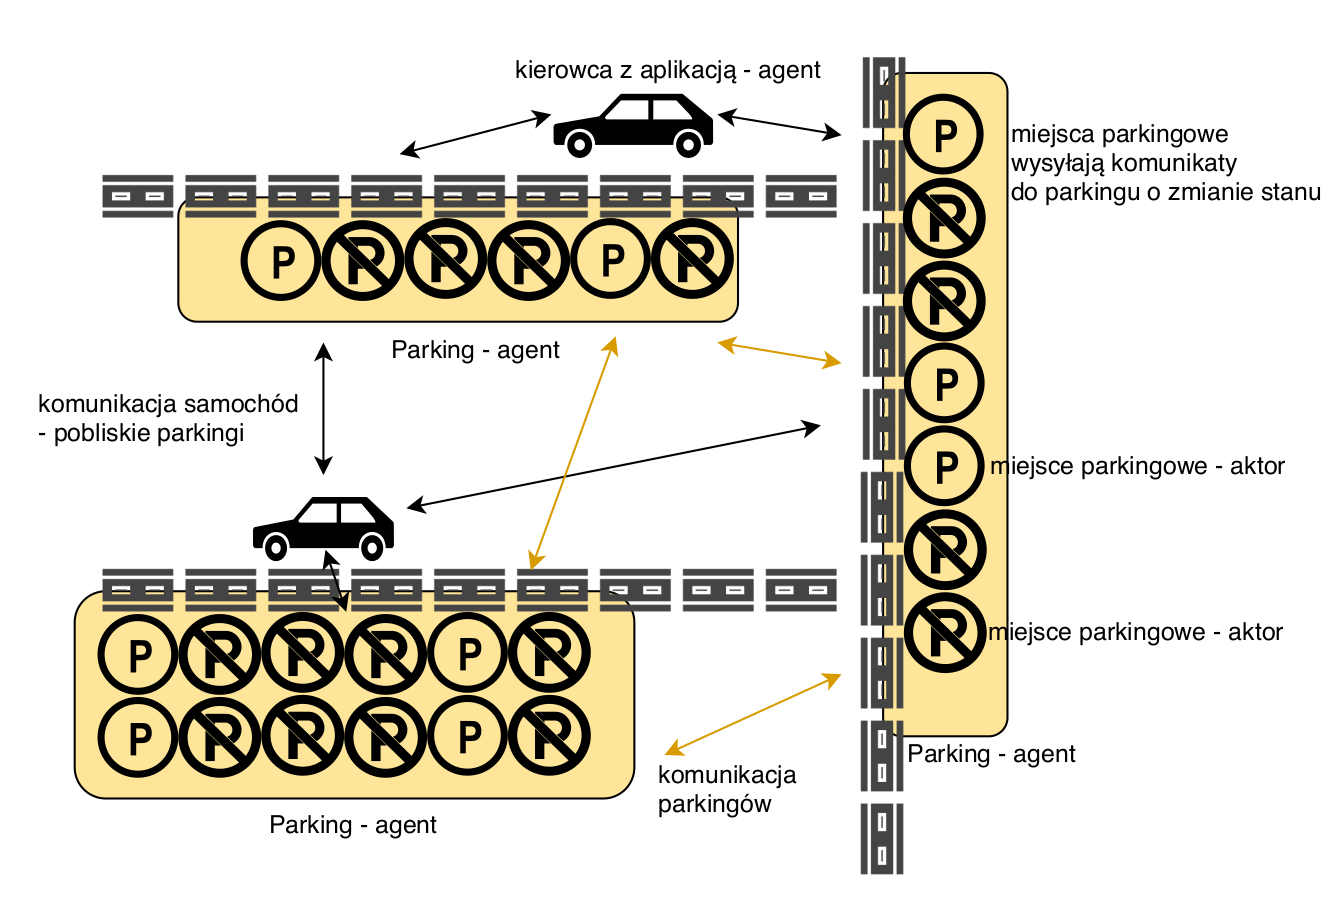
\includegraphics[width=1.1\linewidth]{archi.png}
    \caption{Architektura systemu.}
\end{figure}